\chapter{Resultados}
\label{cap:result}
Para sabermos se o protótipo atingiu nossos objetivos é preciso analisar três pontos importantes: sua capacidade de transmissão em longo alcance juntamente com a eficiência de lidar com altas interferências ao longo do trajeto, seu consumo energético e seu custo de produção. Todo o código fonte desenvolvido neste projeto pode ser acesso em \cite{owlify}.

% ---
\section{Análise de Transmissão dos Pacotes}
\label{result:transmissao}
Foi executado um teste de transmissão de pacotes com o objetivo de verificar a capacidade de transmissão em um longo alcance em um ambiente com altas interferências. O experimento foi realizado no bloco dos professores do IFPB - Campus Campina Grande, onde o \textit{end node} ficou posicionado no laboratório GComPi, localizado no subsolo, enquanto o \textit{gateway} ficou em um espaço diferente, no Laboratório Assert, no térreo do prédio, com cerca de sessenta metros de distância entre os dispositivos, e contanto com obstáculos variados à comunicação, como paredes densas, laje, objetos metálicos e equipamentos eletrônicos. Na figura \ref{fig:experiment-01} podemos ver a distância entre o \textit{gateway} e o \textit{end node}, respectivamente, A e B.

\begin{figure}[H]
  \centering
  \includegraphics[width=.80\textwidth]{assets/experiment-01.png} 
  \caption{Distância aproximadas entre os dispositivos (Adaptada do Google Maps).}
  \label{fig:experiment-01} 
\end{figure}

Os dispositivos ficaram funcionando por cinco dias, 24 horas por dia, realizando envios contínuos de pacotes em intervalos de cinco minutos e o código da análise poder ser acessado em \cite{owlify_lora_transmitter_test}. O gráfico na figura \ref{fig:21-04-2020-pdr-rssi} apresenta a taxa de entrega de pacote, PDR, por horas, das coletas realizadas no dia 21 de abril de 2020. A média geral da PDR foi de 78,82\%, um valor agradável, no entanto, em alguns momentos a PDR ficou em torno de 20\%, o que pode ter sido ocasionado por modificações no perfil de multi-percurso do ambiente, obstáculos temporários ou presença de fontes de interferência. Considerando a taxa de transmissão de pacote utilizada, com PDR de 20\% ainda é possível obter uma nova informação a cada 25 minutos, em média, o que é suficiente para a realização do monitoramento de temperatura e umidade, que são grandezas que variam lentamente.

\begin{figure}[H]
  \centering
  \includegraphics[width=.80\textwidth]{assets/21-04-2020-pdr-rssi.png} 
  \caption{Percentual de entrega dos pacotes em barras e indicador de intensidade do sinal recebido em linha (Autoral).}
  \label{fig:21-04-2020-pdr-rssi} 
\end{figure}

% ---
\section{Análise do Consumo Energético}
\label{result:consumo}
É possível estimar o tempo de duração do \textit{end node} com a bateria escolhida, dividindo a capacidade da bateria pelo consumo de energia médio do dispositivo, e para saber o consumo médio do \textit{node}, precisamos saber o valor do consumo em dois pontos, quando estiver realizando a transmissão de um pacote,  quando estiver em período de espera para a próxima transmissão e o tempo de duração de cada período.

Os dados foram medidos utilizando um multímetro e um osciloscópio, para o primeiro protótipo, entretanto, para o segundo protótipo, devido a dificuldade de acesso aos equipamentos por causa da pandemia do COVID-19, não foi possível realizar a medição de forma manual, e por isso foi utilizado os dados retirados dos \textit{datasheet} dos componentes \cite{datasheetDHT22, datasheetATmega328P, datasheetLoRa}. Para a medição com osciloscópio, foi necessário o uso de um resistor de derivação, também conhecido como resistor \textit{shunt}, de 0,1 Ohm, medindo a queda de tensão diferencial através deste resistor.

O período de coleta que consideramos ser o suficiente para gerar uma boa monitoração é de uma hora e o LoRa demora em torno de 42 ms para realizar uma transmissão de um pacote. Podemos ver na figura \ref{fig:end-node-consumption-chart}, o gráfico mostrando os valores do período de transmissão dos seguintes protótipos para comparação: primeiro protótipo, do segundo protótipo utilizando a função padrão do Arduino, \textit{delay}, e o segundo protótipo em modo \textit{deep sleep} quando estiver em espera, este modo desativa o máximo de funcionalidade do microcontrolador deixa apenas o essencial para voltar ao funcionamento depois de um determinado período. Podemos ver, o consumo em espera e quando está realizando uma transmissão, respectivamente, para o primeiro protótipo, temos 50 ms e 150 ms, já para o segundo protótipo utilizando o\textit{delay}, temos 18 ms e 118 ms e para o segundo protótipo em modo  \textit{deep sleep}, temos os menos valores, com 0.06 ms e 118 ms.

\begin{figure}[H]
  \centering
  \includegraphics[width=.80\textwidth]{assets/end-node-consumption-chart.png} 
  \caption{Gráfico de consumo dos protótipos do \textit{end node} (Autoral).}
  \label{fig:end-node-consumption-chart} 
\end{figure}

Com esses dados, é possível calcular a corrente média somando os valores de medida multiplicados pelas suas porcentagens referentes ao tempo total. O tempo total do período equivale a 3600,042 s, que corresponde à soma do tempo em transmissão, 42 ms, com o tempo em espera, 3600 s. Temos então 56.0010904 mA para o primeiro protótipo, 18.00116 mA para o segundo utilizando \textit{delay} e 0,06136 mA para o segundo em modo \textit{deep sleep}, como é possível ver nas equações \ref{equation:p1-consumption}, \ref{equation:p2-consumption} e \ref{equation:p3-consumption}, respectivamente.

\begin{equation}
  (0,9999884 * 56 mA) + (0,0000116 * 150 mA) = 56,0010904 mA
  \label{equation:p1-consumption} 
\end{equation}

\begin{equation}
  (0,9999884 * 18 mA) + (0,0000116 * 118 mA) = 18,00116 mA
  \label{equation:p2-consumption} 
\end{equation}

\begin{equation}
  (0,9999884 * 0,06 mA) + (0,0000116 * 118 mA) = 0,06136 mA
  \label{equation:p3-consumption} 
\end{equation}

Agora, com esses dados, podemos calcular a duração teórica dos protótipos  para uma bateria, no nosso caso a 18650, com 2200 mAh, que é aproximadamente 39 horas para o primeiro protótipo, 122 horas para o segundo protótipo utilizando \textit{delay} e 35.849 horas para o segundo protótipo utilizando \textit{deep sleep}, como mostra nas equações \ref{equation:p1-hours}, \ref{equation:p2-hours} e \ref{equation:p3-hours}.

\begin{equation}
  \frac{2200 mAh}{56,0010904 mA} = 39,2849494 h
  \label{equation:p1-hours} 
\end{equation}

\begin{equation}
  \frac{2200 mAh}{18,00116 mA} = 122,214346 h
  \label{equation:p2-hours} 
\end{equation}

\begin{equation}
  \frac{2200 mAh}{0,06136 mA} = 35.849 h
  \label{equation:p3-hours} 
\end{equation}

% ---
\section{Análise do Custo}
\label{result:custo}
Todas as compras dos equipamentos foram realizadas no Brasil e em baixa quantidade, o que acaba deixando o protótipo mais caro comparado a compra realizada na China ou comprando em grande escala, que acaba tendo uma redução considerável do seu custo. Tendo isto em mente, podemos analisar a tabela \ref{tab:costs-2-proto}, representando o custo (sem consideração do frete), da cada peça encontrada no Brasil e na China para montar o segundo protótipo do \textit{end node} apresentado na sessão \ref{metod:end-node:2-proto}. Os dados da tabela foram preenchidos com os menores valores encontrados no dia 11 de abril de 2021 considerando os revendedores mais confiáveis. Temos então, um total de R\$ 97,66 comprando localmente e R\$ 48,40 importando, que dá em torno de 49,56\% a menos comprando na China, tornando assim um melhor custo benefício.	Já para o \textit{gateway}, o preço no Brasil fica em torno de R\$ 180,00 e importando pode ser encontrado por menos de R\$ 100,00.

Considerando que, ao utilizar um produto deste porte, não será mais necessário a compra de câmeras conservadoras com monitoração, que pode chegar a custar R\$ 10.000,00, podendo assim, economizar até R\$ 7.000,00 por refrigerador, tornando o nosso produto viável financeiramente para as empresas.

\begin{table}[H]
  \centering 
  \scalebox{1} {
    \begin{tabular}{l | l | l}
    \textbf{Componente}&\textbf{Preço no Brasil}&\textbf{Preço na China}\\[5pt] \hline
    &&\\
    Um ATmega328&R\$ 19,90&R\$ 9,12 \\[5pt]
    Um LoRa RFM95W 915 Mhz&R\$ 56,00&R\$ 20,99 \\[5pt]
    Um Bateria 18650 3000 mAh&R\$ 19,90 &R\$ 17,65 \\[5pt]
    Um Cristal Oscilador 1 6mhz&R\$ 01,47&R\$ 00,46 \\[5pt]
    Um Capacitor de cerâmica 100pF&R\$ 00,05&R\$ 00,04 \\[5pt]
    Dois Capacitor de cerâmica 22pF&R\$ 00,22&R\$ 00,08 \\[5pt]
    Dois Resistores de 10 kOhms&R\$ 00,12&R\$ 00,06 \\
    &&\\ \hline
    &&\\
    \textbf{Total}&R\$ 97,66&R\$ 48,40 \\[5pt]
    \end{tabular}
  }
  \caption{Custos referente as peças do segundo protótipo do \textit{end node} (autoral).}
  \label{tab:costs-2-proto}
\end{table}

Temos então os preços dos protótipos da parte física, os hardwares, é preciso agora, calcular o custo da publicação do aplicativo na \textit{Play Store}, loja de aplicativos da Google, e o custo de hospedagem do servidor. Para a publicação do aplicativo é mais simples, a Google cobra apenas um valor fixo para poder realizar qualquer publicação na loja de US\$25,00, em torno de R\$ 131,56 na cotação do dia 17 de maio de 2021.

Por fim, temos o custo da hospedagem do servidor, essa é um valor mensal que varia conforme a demanda de processamento, armazenamento e transferência de dados, e também é diferente para cada provedor. Dentre os diversos provedores, os mais conhecidos são: Amazon Web Services, Google Cloud, Microsoft Azure e DigitalOcean.

A DigitalOcean oferece em seu site, uma calculadora que compara o custo em dólares estadounidenses por mês, entre os provedores citados, conforme a configuração do servidor desejada \footnote{https://www.digitalocean.com/pricing/calculator/}. Inicialmente, a melhor configuração é a básica, pois a demanda de serviço é baixa, com o tempo, basta aumentar de acordo com o crescimento da demanda. Tendo isto em mente, levei em consideração a configuração básica e a de propósitos gerais fornecida pela DigitalOcean, os dados podem ser vistos na figura \ref{fig:server-chart}.

\begin{figure}[H]
  \centering
  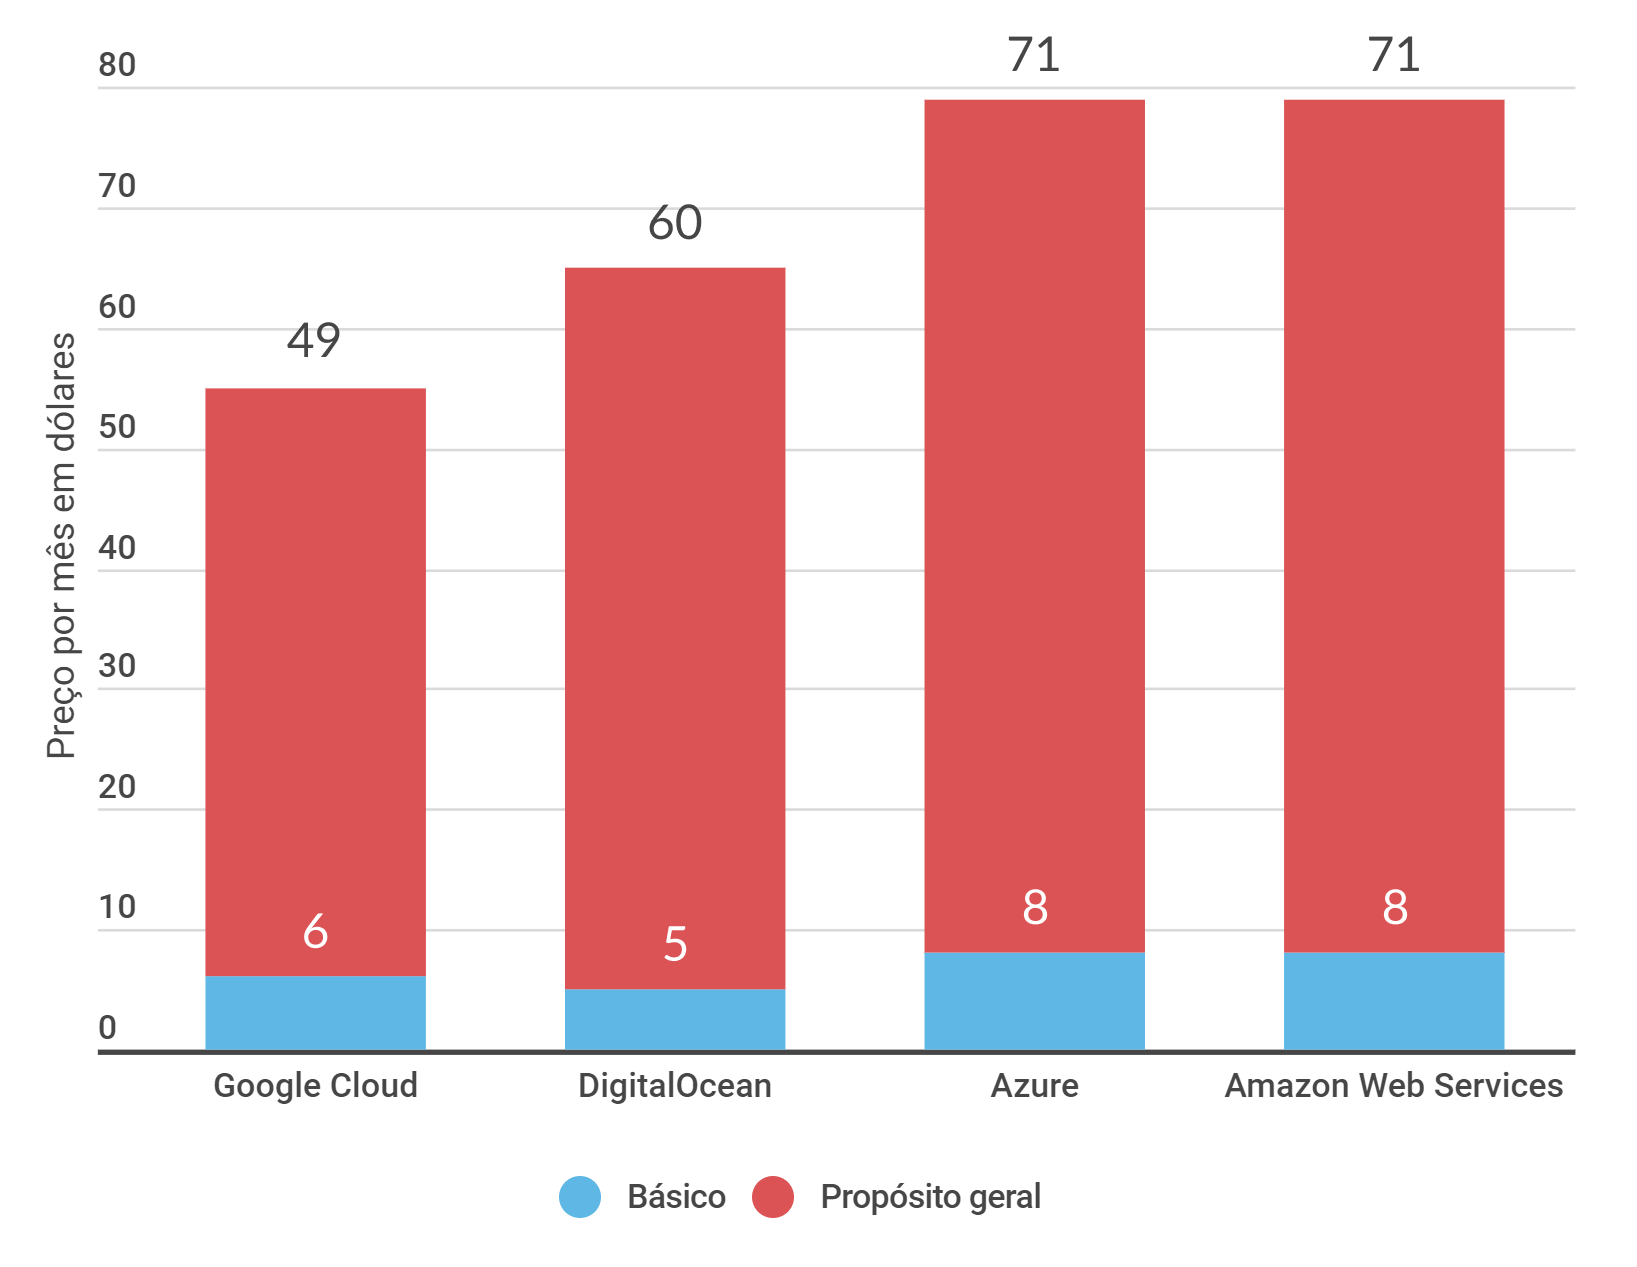
\includegraphics[width=.80\textwidth]{assets/server-chart.png} 
  \caption{Comparação do custo mensal de hospedagem do servidor (Autoral).}
  \label{fig:server-chart} 
\end{figure}

Na configuração básica, a DigitalOcean é a opção mais barata, custando US\$5,00, seguido pela Google Cloud por US\$6,00. Já na configuração de propósitos gerais, temos uma inversão, a mais barata fica com a Google Cloud por US\$49,00 seguida pela DigitalOcean por US\$60. Entretanto, conforme aumenta a demanda, acaba com a DigitalOcean ficando na frente, além dela prover uma boa usabilidade.